\documentclass[a4paper,12pt]{article}

\usepackage[utf8]{inputenc}
\usepackage[lmargin=3cm,tmargin=3cm,rmargin=2cm,bmargin=2cm]{geometry}
\usepackage[onehalfspacing]{setspace}
\usepackage{blindtext}
\usepackage[T1]{fontenc}
\usepackage[brazil]{babel}
\usepackage[document]{ragged2e}

\usepackage{graphicx, xcolor, comment, enumerate, multirow, multicol}
\usepackage{indentfirst}

\usepackage{amsfonts, amsthm, amsmath, amssymb, dsfont, mathtools}
\usepackage{tikz, tkz-base, tkz-fct}
\usepackage[style=abnt]{biblatex}

\newcommand{\PR}[1]{\ensuremath{\left[#1\right]}}
\newcommand{\PC}[1]{\ensuremath{\left(#1\right)}}
\newcommand{\chav}[1]{\ensuremath{\left\{#1\right\}}}
\newcommand{\system}[1]{\ensuremath{\left\{#1\right}}

% Citacao direta com mais de 3 linhas - ABNT NBR 10520/2002 - 5.3
\newlength{\ABNTEXcitacaorecuo}% recuo de 4 cm da margem esquerda
\setlength{\ABNTEXcitacaorecuo}{4cm}
\newcommand{\ABNTEXfontereduzida}{\footnotesize}
\newenvironment*{citacao}[1][default]{%
   \list{}%
   \ABNTEXfontereduzida%
   \addtolength{\leftskip}{\ABNTEXcitacaorecuo}%
   \item[]%
   \singlespacing
   \ifthenelse{\not\equal{#1}{default}}{\itshape\selectlanguage{#1}}{}%
 }{%
   \endlist}%
% ---

\newenvironment{invisible}{\color{white}}{}
\usepackage{booktabs}

\addbibresource{ref.bib}

\begin{document}

\begin{minipage}{.1\linewidth}
    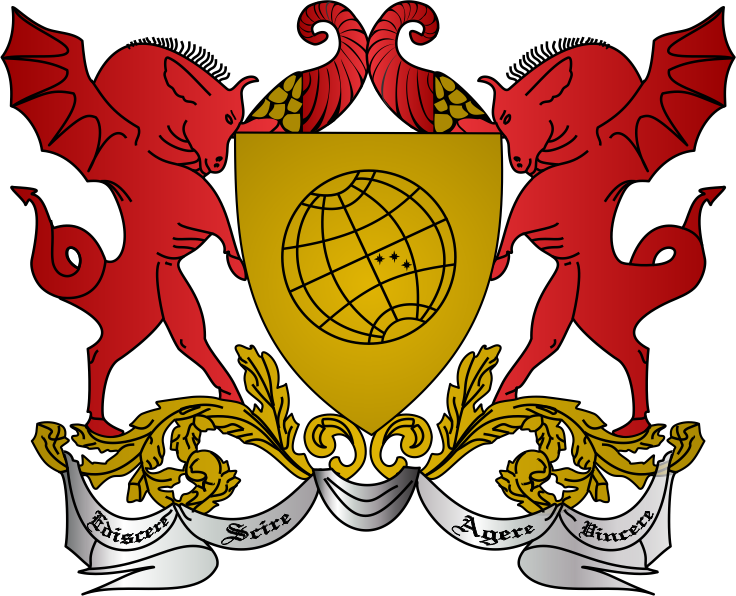
\includegraphics[width=3cm]{ufv2.png}
\end{minipage}
\begin{minipage}{.9\linewidth}

\thispagestyle{empty}

\begin{center}
\textbf{UNIVERSIDADE FEDERAL DE VIÇOSA}

CENTRO DE CIÊNCIAS HUMANAS, LETRAS E ARTES

DEPARTAMENTO DE ECONOMIA
\end{center}
\end{minipage}


\vspace{4cm}

\begin{center}

    \textbf{UMA ANÁLISE DE THOMAS KANG SOBRE A EDUCAÇÃO PRIMÁRIA NO BRASIL, 1930-1964. (RESENHA)}
\end{center}

\vspace{4cm}

\begin{flushright}
DISCENTE: FLÁVIO HUGO PANGRÁCIO SILVA.

\vspace{0.5cm}

DOCENTE: GIOVANA FIGUEIREDO  ROSSI.
\end{flushright}

\vspace{6cm}

\begin{center}

VIÇOSA

MINAS GERAIS - BRASIL

\textbf{Agosto/2021}
    
\end{center}

\newpage

\thispagestyle{empty}

\tableofcontents

\newpage

\section*{Resumo}
\addcontentsline{toc}{section}{Resumo}

\justifying

O Brasil tem apresentado, ao longo de sua história, resultados educacionais pífios em relação aos seus vizinhos latino-americanos.
A literatura sugere que uma possível causa do atraso educacional tenha sido o viés elitista das políticas educacionais. \cite{kang}.

O trabalho do professor Thomas Kang traz evidências de que as políticas educacionais conduzidas pelo governo federal foram elitistas no período 1930–1964.

Segundo Kang \cite*{kang}, embora o ensino primário fosse responsabilidade dos estados,
grande parte das receitas tributárias estava sob o poder da União. Assim, as políticas educacionais federais eram importantes para determinar os resultados em todos os níveis de ensino.
As evidências coletadas em discursos e em dados de financiamento educacional mostram que as políticas do período tenderam a dar pouca importância ao ensino primário.
Em particular, há evidências de que os governos de Getúlio Vargas e Juscelino Kubitschek, os mais compromissados com a estratégia de industrialização por substituição de importações, privilegiaram o ensino superior, em detrimento do ensino primário para as massas.

\section*{Introdução}
\addcontentsline{toc}{section}{Introdução}

Apesar do Brasil ser o maior país da América Latina em extensão geográfica e tamanho populacional,
foi deixado de lado por pesquisadores como Stanley Engerman e Kenneth Skoloff \cite*{NBERenge11-1,NBERh0066},
que realizaram estudos sobre as origens das desigualdades entre as Américas.
Em um capítulo específico, falam sobre o atraso educacional e analisam o histórico da educação de vários países latinos,
e mais uma vez, o Brasil nem é citado, muito, talvez, pela insuficiente base de dados históricos da educação. A escassez de dados não são muito animadores.
Em 1950, cerca de 50\% da população brasileira era analfabeta \cite{kang}.
No mesmo período, as taxas de matrícula e os anos de escolaridade média eram menores que aos apresentados por países vizinhos como Argentina ou Bolívia \cite{astorga}.


\begin{citacao}
    Apesar dos avanços desde então, como a universalização do ensino fundamental na década de 1990, o Brasil continua registrando dados pouco alentadores em termos comparativos. Os resultados brasileiros no Programme of International Student Assessment (PISA), exame de proficiência escolar promovido pela Organização para Cooperação e Desenvolvimento Econômico (OCDE), costumam classificar o país nas últimas posições dentre os países participantes (Organisation for Economic Cooperation and Development 2013). \cite{kang}
\end{citacao}

Ben Ansell \cite*{ansell_2010}, apresenta uma explicação para o insucesso da educação básica em diversos contextos, incluindo o Brasil.
Ele diz que, a opção por uma estratégia de industrialização por substituição de importações, com pequeno grau de abertura da economia ao exterior, teria gerado desincentivos a melhorias na educação para as massas.
Pois, em economia mais fechadas, o aumento da oferta de trabalho qualificado levaria a uma diminuição maior dos rendimentos relativos do trabalho qualificado, o que geraria incentivos para a manutenção de políticas educacionais excludentes.\footnote{A expansão educacional em economias abertas tende a gerar mudanças na composição da produção (efeito Rybczynski), utilizando mais intensivamente a oferta de trabalho qualificado (agora mais abundante) em suas economias, com menores consequências sobre os salários dos mais qualificados (resultado conhecido como equalização ou insensibilidade dos preços dos fatores).}

Kang \cite*{kang}, concorda com Ansell e afirma que, de maneira geral, as políticas educacionais
priorizaram o ensino superior e secundário para as elites, em detrimento do ensino primário para as massas, ao longo do período 1930-1964.
Afirma também, que os governos desse período são objetos de diversas controvérsias com relação ao seu papel na redução da pobreza e na legislação social e trabalhista.

Com a ascenção de Vargas na década de 30, o governo federal passou a deter grande parte dos recursos financeiros do país. Nesse contexto, Kang \cite*{kang} argumenta que os governos do período não quiseram investir na melhoria do ensino primário para as massas no Brasil entre 1930 e 1964.
Dessa forma, ao responsabilizar as unidades federativas pela provisão de ensino primário, as elites políticas nacionais, aceitaram que o ensino primário permanecesse atrasado com relação aos países latinos.

\section*{A evolução do ensino primário no Brasil, 1930-1964}
\addcontentsline{toc}{section}{A evolução do ensino primáro no Brasil, 1930-1964}

Entre 1930 e 1964, a economia brasileira alcançou um crescimento médio de 5,6\% a.a, e a expansão média do PIB per capita foi de 3,2\% a.a.
O setor industrial passou a ser responsável por cerca de 25\% do vaor adicionado bruto em 1950, chegando à 33\% em 1964. A população aumentou de 35 milhões em 1930, para cerca de 70 milhões na década de 1960.
Além disso, acontece um intenso movimento migratório para os centros urbanos: A taxa de população residente na zona urbana que era de 31\% em 1940, passou para 56\% nos anos 70. \cite{kang}.

Em relação à educação, houve mudanças na política educacional entre os diferentes regimes. No entanto, o que marca esse período é a persistência no atraso educacional.
De acordo com os censos demográficos, 56\% da população com mais de 15 anos de idade eram analfabetos em 1940.
Essa taxa caiu para 50,5\% em 1950, e para 39,5\% em 1960, chegando a 33,6\% em 1970 (IBGE, 2000).
Alguns países latinos, como México e Venezuela, tiveram a mesma velocidade da queda de analfabetismo nos anos 50, seguindo o mesmo atraso do Brasil. \cite{frankema}.

Os dados de matrícula contidos nos censos demográficos revelam outras informações (IBGE 1900–1970). Cerca de 25,5\% da população entre 5 e 14 anos estava matriculada em escolas em 1940.
Diminuindo para 24,1\% em 1950, e aumentando para 41,9\% em 1960. Logo, embora tenha havido uma melhora em 1960, mais da metade das crianças nessa faixa etária estava fora da escola no final do período estudado.

\begin{citacao}
Embora as matrículas tenham crescido,
é possível atribuir essa elevação a outras variáveis,
como aumento da urbanização e da renda,
e não a políticas educacionais inclusivas.
Argumento em seções posteriores que foi esse o caso,
principalmente observando os discursos dos governos e o padrão de financiamento,
ambos mais voltados ao ensino superior. \cite[p. 38]{kang}.
\end{citacao}

\begin{citacao}
    Além disso,
    observar o comportamento de determinados governos dentro de um mesmo regime político pode oferecer pistas adicionais sobre se houve ou não priorização do ensino primário.
    Apesar da continuidade em diversos aspectos,
    houve diferenças importantes dentro do mesmo regime político.
    Durante os primeiros anos do Governo Vargas,
    nas fases do Governo Provisório e do Governo Constitucional,
    ocorreu uma substancial expansão de matrículas em termos nacionais.
    \cite[p. 38]{kang}.
\end{citacao}

    Durante o regime autoritário do Estado Novo,
    principalmente nos anos da Segunda Guerra Mundial,
    o percentual de matrícula no primário caiu.
    A taxa de matrícula,
    que era de 54,9\% em 1940,
    diminuiu para 52,1\% em 1944,
    seguida por uma recuperação marginal em 1945 (52,9\%). \cite{kang}.



\begin{table}[h!]
    \caption{Taxas médias de crescimento econômico e crescimento da taxa de matrícula bruta no ensino primário fundamental comum por governo, Brasil, 1930–1964.}

    \vspace{0.3cm}

    \label{tabela1}
    \begin{tabular}{@{}llcc@{}}
    \toprule
    \textbf{Governo} &
      \textbf{Período} &
      \textbf{\begin{tabular}[c]{@{}c@{}}Taxa média de crescimento\\ econômico (\%)\end{tabular}} &
      \textbf{\begin{tabular}[c]{@{}c@{}}Taxa média de crescimento \\  da taxa de matrícula(\%)\end{tabular}} \\ \midrule
    Vargas     & 1930-1937 & 4,59 & 4,95  \\
    Vargas     & 1938-1945 & 3,44 & -0,15 \\
    Dutra      & 1945-1950 & 7,64 & 4,30  \\
    Vargas     & 1951-1954 & 6,18 & 1,73  \\
    Kubitschek & 1956–1960 & 8,12 & 2,57  \\
    Goulart    & 1962-1964 & 3,60 & 6,11  \\ \bottomrule
    \end{tabular}

    \vspace{0.3cm}

    \scriptsize{Fonte: Haddad (1978) e IBGE, Anuário estatístico do Brasil (vários anos), citado por Kang \cite*{kang}.}
\end{table}
É possível ver, mediante os dados (Tabela \ref{tabela1}), as divergências entre as políticas educacionais de diferentes governos no período democrático.
É evidente a acentuada elevação da taxa de matrícula bruta durante os governos de Dutra e João Goulart (4,3\% e 6,11\%, respectivamente), comparados com os governos de Vargas e JK.
Além disso, é nítida a diferença dentro da Era Vargas: 4,95\% na fase Provisória e Constitucional \textit{versus} -0,15\% da fase autoritária (Estado Novo).
Dessa maneira, não é difícil associar o comportamento dessas variáveis com base nos discursos presidenciais,
políticas efetivamente implementadas e nos recursos financeiros destinados ao ensino primário durante os mandatos desses governos.


\section*{O ensino primário na Era Vargas: 1930-1945}

Antes de assumir o poder, o ensino primário sempre esteve em segundo plano na campanha de Vargas.
O documento de campanha da Aliança Liberal de Vargas (1938, p.25 apud Kang (2017)) afirmava que "tanto o ensino secundário quanto o superior reclamam alterações [...] que não comportam adiamento".
Não havia a mesma urgência para o caso do ensino primário. Após ser derrotado nas eleições de 1930,
Vargas chegou ao poder através de um golpe.

Uma de suas primeiras medidas foi a criação do Ministério da Educação e da Saúde Pública em 1930.
O cargo foi ocupado por Francisco Campos,
que empreendeu reformas no ensino,
introduzindo disciplinas de caráter técnico-científico no secundário e aumentando a interferência do governo na educação. \cite{capanema}.

No primeiro ano do governo provisório,
Vargas (1938, p.228-229 apud \cite{kang}) reconheceu que “em matéria de educação nacional, quase tudo está por fazer-se”, e segundo Kang \cite*[p. 39]{kang}, dedicou "[...] apenas dezesseis linhas ao assunto instrução primária e técnico-profissional".
Mas era o ensino secundário que “requeria urgente reforma” (Vargas 1938, p. 229 apud \cite{kang}).
Na mensagem à Assembleia Constituinte de 1933,
Vargas (1938, p. 124–125, p. 128–129 apud \cite{kang}) novamente reconhecia a educação primária como “magno problema”,
relatando casos de sucesso como Japão e Estados Unidos e o atraso brasileiro.
No entanto, seu discurso não passou do diagnóstico do problema do ensino primário,
enquanto anunciava a elaboração de uma proposta clara para reforma do ensino secundário (Vargas 1938, p. 130–132 apud \cite{kang}).
Ao listar, em junho de 1934, as realizações educacionais do governo até então, Vargas (1938, p. 134 apud \cite{kang}) destacou a criação de inúmeras faculdades.
Em relação ao ensino primário, a única realização foi a criação da Taxa de Educação e Saúde.

Uma nova constituição foi redigida, ainda em 1934, com uma orientação bastante favorável à uma centralização em diversas áreas de atuação do Estado,
incluíndo a política educacional. Sob influência do novo ministro da educação,
Gustavo Capanema, e da Escola Nova, movimento pedagógico renovador da época,
a Constituição de 1934 deu competência à União para “traçar as diretrizes da educação nacional”,
além de coordenar e fiscalizar o ensino em geral. Além disso, foi fixado o Plano Nacional de Educação.
O ensino primário foi declarado gratuito e de frequência obrigatória.
União e municípios foram obrigados a aplicar pelo menos 10\% de seu orçamento à educação,
enquanto estados e Distrito Federal deveriam investir no mínimo 20\% \cite{silva}. A Constituição de 1934 também ressaltava a ação supletiva da União em matérias educacionais onde havia “deficiência de iniciativa ou de recursos” (artigo 150).
Essa abertura não excluía o envolvimento da União no financiamento do ensino primário, algo que já estava inscrito na Constituição de 1891. \cite{kang}.

A constituição liberal-democrática de 1934, no entanto, não durou muito. Pois, em 1937,
Vargas fechou o Congresso, dando início à repressiva, centralizadora e corporativista ditadura do Estado Novo.

No mesmo ano, foi outorgada uma nova constituição que,
na prática, representou um passo atrás em relação à Constituição de 1934 em matéria educacional.
Mais preocupada com a educação voltada à ideologia nacionalista do Estado Novo, a nova constituição fez poucas referências ao ensino em geral.
A Constituição do Estado Novo claramente colocava como objetivo a industrialização do país e, assim, o ensino industrial ganhou destaque e a educação aparece apenas como instrumento das políticas industriais.
\cite{kang}

A atuação de Gustavo Capanema no ministério de educação e saúde, marcou a política educacional do Estado Novo.
Apesar de dar certa importância ao ensino primário, Capanema entendia que o governo federal não poderia supervisionar esse nível de ensino,
cuja responsabilidade deveria ser dos governos estaduais.
Os estados deveriam coordenar o ensino primário, ao passo que à União caberia a cooperação supletiva, a assistência técnica e o estabelecimento de diretrizes gerais. \cite{Quadros_Machado_2013}

Capanema acreditava que a formação de uma elite que liderasse o país era a tarefa mais importante, pois seria condição suficiente para o progresso nacional. \cite{capanema}.

\begin{citacao}
A Lei Orgânica do Ensino Secundário e a Lei Orgânica do Ensino Industrial, que organizaram essas categorias de ensino, foram decretadas em 1942. Com relação ao ensino secundário, a reforma de Capanema voltou-se ao predomínio da formação clássica e humanística, uma vez que era voltada à formação da elite. \cite[p. 40]{kang}.
\end{citacao}

\section*{O ensino primário no regime democrático, 1945-1964}

Com a redemocratização, marcada pelo fim do Estado Novo, fez-se necessária a construção de uma nova constituição federal.
A Constituição aprovada em 1946 recuperou os princípios da Constituição de 1934: retomou-se a provisão mínima de recursos destinados à educação, fixada em 10\% para União e estados e em 20\% para municípios.
Além disso, a Constituição definiu a necessidade de uma legislação de diretrizes e bases da educação nacional.
Tal Constituição, também afirmava o papel supletivo da União em matéria de ensino primário,
mas ressaltava a necessidade de auxílio pecuniário da União por meio dos Fundos Nacionais aos estados e ao Distrito Federal.
\cite{kang}.

Durante o governo Dutra, houve certa tendência de melhora nos indicadores educacionais. Kang \cite*{kang} diz: "O posicionamento favorável de Dutra quanto à expansão educacional é até surpreendente, dado o caráter repressivo de seu governo em muitos aspectos, particularmente em relação aos sindicatos".
Desde o tempo do Estado Novo, Dutra já mostrava preocupação com a situação do ensino primário ao criticar a política nacionalista para a juventude proposta por Francisco Campos. Para Dutra, não fazia sentido um ensino cívico, sem antes uma solução para o analfabetismo. \cite{capanema}.

Nesse trecho, Kang \cite*[p. 40-41]{kang}, cita diversos discursos de Dutra:

"Os relatórios presidenciais de Dutra (1947, 28–35) mostram que, pelo menos no discurso, a questão da educação popular era prioritária. De acordo com o Relatório Presidencial de 1947, não menos importante que o problema econômico era “o da educação, a que, em minhas manifestações de candidato, reconheci aquêle primacial relevo que o torna em preocupação constante do meu governo” (Dutra 1947, 16). E ainda continuava Dutra (1947, 18): “É mister dar a cada brasileiro igualdade de oportunidade, a começar pelo ensino primário, extensivo aos adultos, tanto mais quanto nossa população escolar vem apresentando nos últimos anos progressivo declínio”. Dutra ressaltou em seu primeiro relatório que 50 por cento da arrecadação da Taxa de Educação e Saúde, criada em 1931, não recebiam emprego específico, o que teria sido corrigido: 75 por cento das receitas passaram a ser empregadas no FNEP (Dutra 1947, 30). O Presidente ainda destacou o financiamento de 2.270 escolas rurais, das quais 500 já terminadas e mil estariam em fase adiantada de conclusão (Dutra 1948, 55); de 10.416 classes de educação para adultos em 1947 e 14.119 em 1948 (Dutra 1949, 117); e da construção de 4.360 prédios escolares, dos quais mil teriam sido concluídos (Dutra 1949, 119). Em 1949, estaria encaminhada a construção de 6.160 prédios, dentre os quais 3.000 teriam sido concluídos (Dutra 1950, 115)."

Os dados do período governado por Dutra mostram crescimento da taxa de matrícula bruta no ensino primário fundamental público: a taxa era de 52,9\% em 1945, enquanto que, em 1950, esta taxa atingiu 64,8\%.
A taxa de crescimento média das matrículas do ensino primário fundamental público durante o governo Dutra foi de 4,3\%, contrastando com a média de 2,1\% do período 1950–1955 (Vargas e Café Filho) e com os 2,6\* do governo Juscelino Kubitschek no período 1956–1961. \cite{kang}.

Depois da surpreendente atuação de Dutra, os anos 1950 foram marcados pelo pouco caso ao ensino primário. De acordo com Bomeny (2008 apud Kang (2017)), o segundo governo Vargas (1951–1954) fez muito pouco pela educação, resumindo-se à criação de órgãos administrativos superiores como o Conselho Nacional de Pesquisa em 1951, a Campanha Nacional de Aperfeiçoamento de Pessoal de Nível Superior (CAPES) também em 1951 e a Campanha de Aperfeiçoamento e Difusão do Ensino Secundário.
Como se pode ver na (Tabela \ref{tabela1}), há uma brusca queda na taxa de crescimento de matrículas.

Após o suicídio de Vargas, e um pequeno período de transição (Café Filho 1954-1955), Kubitschek é eleito presidente em 1955, tomando posse em 1956.
Seu governo é geralmente lembrado como símbolo de progresso, devido ao intenso crescimento econômico liderado pela indústria de bens de consumo duráveis.
Por outro lado, o governo de Kubitschek é um exemplo da ausência de prioridade no ensino primário.\cite{kang}.

Durante o mandato de Kubitschek (1956–1961), atingiu-se a taxa de crescimento econômico média mais alta do período 1930–1964: a economia brasileira cresceu em média 8,1\% ao ano.
Ao longo dos anos JK, a dívida externa líquida aumentou 50\%, como resultado da política de incentivo à entrada de capital estrangeiro.
Os déficits públicos, a política monetária expansionista e o rápido crescimento, por sua vez, levaram a uma inflação média de 24,7\% ao ano.
Foi, portanto, uma política de crescimento acelerado mas com elevado custo, por não contar com mecanismos eficientes de financiamento. \cite{kang}.

A educação, considerada um dos alicerces do crescimento econômico de longo prazo, não esteve no centro das políticas públicas no governo JK, de forma coerente com o restante da política econômica, que estava concentrada nos resultados de curto prazo.\footnote{Mais detalhes em Aula 4, da Professora Giovana. F . Rossi.}

Pós JK, tivemos um pequeno e conturbado período de governo Jânio Quadros, que terminou com uma renúncia. O vice Jõao Goulart assumiu a presidência.

Jõao Goulart, sob o presidencialismo, nomeou o educador Darcy Ribeiro como ministro da educação e propôs, no Plano Trienal, o aumento das despesas mínimas com educação da União de 10\% para 15\% em 1964 e para 20\% em 1965.

\begin{citacao}
    No Plano Trienal proposto pela equipe econômica (Celso Furtado e San Tiago Dantas) de Goulart em 1963, enfatizou-se a importância instrumental do ensino primário para o crescimento econômico. Por esse motivo, reconhecendo as dificuldades que possivelmente alguns estados e municípios enfrentavam para investir recursos suficientes no ensino primário, caberia “à União compensar a incapacidade financeira dos governos locais nas regiões de menor grau de desenvolvi- mento econômico” (Brasil, Presidência da República, 1962, 87). \cite{kang}.
\end{citacao}

Os dados do período confirmam a maior ênfase dada pelo governo Goulart: no período 1962–1964, a taxa média anual de crescimento da taxa de matrícula bruta no ensino fundamental público foi de 6,1\%, a maior dentre os governos democráticos após o fim do Estado Novo. \cite{kang}.


\section*{Considerações finais de Kang (2017)}

Mesmo com uma estratégia de industrialização acelerada, os governos brasileiros tinham poucos incentivos para investir em uma política redistributiva custosa tanto no curto (custo de oportunidade do gasto público em educação para as massas) como no longo prazo (por meio da redução do prêmio salarial do trabalhador qualificado), principalmente no contexto de economia baseada em elevada proteção comercial. Talvez não por acaso, os governos claramente empenhados na estratégia de ISI deram menor atenção ao ensino primário para as massas. Entre 1930 e 1964, os governos federais que mais apoiaram o ensino primário eram os menos compromissados com a ISI.

De modo geral, todavia, persistiu a orientação elitista dos gastos públicos em educação, com o privilégio deliberado do ensino superior. A centralização política a partir da Revolução de 1930 implicou mudanças nas políticas educacionais com a criação do Ministério da Educação e da Saúde Pública e as reformas do ensino promovidas pelo seu ministro Francisco Campos. Gustavo Capanema, que assumiu o posto em 1934, também empreendeu reformas e priorizou o ensino secundário e superior, com vistas a formar a elite do país. Capanema afirmava que o ensino primário estava a cargo dos estados, mas esses sabidamente viviam em penúria financeira.

A ênfase no ensino das elites transparece nos dados de matrículas. Durante o Estado Novo, período mais centralizado e fechado politicamente, houve até queda na taxa de matrículas no ensino primário. A volta da democracia em 1945, porém, veio acompanhada de aumento das matrículas no ensino primário comum. Em particular, o governo Dutra obteve alguns avanços no ensino primário, como atestam suas declarações e realizações. Entretanto, os governos seguintes de Getúlio Vargas e Juscelino Kubistchek pouco fizeram pelo ensino primário, dando maior importância e direcionando maiores investimentos ao ensino secundário e superior. Apesar da queda nas taxas de crescimento econômico, o período Goulart presenciou um relativo retorno da importância do ensino primário, conforme indicam as estatísticas de matrículas.
46 Educação para as elites

Pode-se argumentar que houve alguma melhoria no ensino primário durante o período. De fato, houve progresso na década de 1950 com relação à alfabetização: de uma proporção de analfabetos que ultrapas- sava os 50 por cento da população de quinze anos ou mais em 1950, o analfabetismo reduziu-se para 39,6 por cento em 1960. Entretanto, esse resultado foi influenciado mais pela expansão do ensino supletivo do que por melhoras no ensino primário comum para crianças, segundo os dados oficiais (IBGE 1933–1971). Ademais, os progressos verificados nas matrículas não despontaram em comparação com outros países latino-americanos.

Parece claro que as poucas ações em favor do ensino primário por parte da maioria dos governos após 1930 não podem ser meramente explicadas por esse nível de ensino ser de responsabilidade constitucional dos estados. O que apresentamos neste trabalho são evidências preliminares de que, em nível federal, as políticas implementadas tenderam a ser elitistas, concentrando-se no ensino secundário e universitário e omitindo-se em relação à situação do ensino primário. Essa evidência sugere que o maior interessado na questão, o segmento populacional majoritário que não fazia parte da elite, não foi capaz de pressionar, de maneira efetiva, o governo federal em favor da ampliação dos direitos educacionais. Em várias ocasiões, as ações tomadas pelo governo federal reforçaram a desigualdade no acesso à educação básica.

Não temos como concluir com base nessas evidências se as políticas favoráveis ao ensino primário pro- movidas por Dutra (1946–1951) e Goulart (1961–1964) foram respostas a demandas da população ou result- antes do compromisso desses governos com a oferta de educação para as massas. É verdade que, em ambos os governos, houve intensa mobilização política nos períodos de maior expansão educacional. O governo Dutra adotou política repressiva contra os sindicatos de trabalhadores, suprimindo a voz política desse grupo em diversas manifestações logo após a volta da democracia. O período de Goulart foi um dos períodos mais conturbados da histórica brasileira, em que o governo propôs numerosas reformas sociais, levando a intensa polarização política. A agenda de pesquisa, portanto, inclui entender a importância das forças de oferta e demanda por educação e a economia política do período, a fim de se compreender melhor os fatores-chave responsáveis pelo atraso educacional brasileiro.

\section*{Objetivos deste trabalho}
Estudar alguma questão que não foi apresentada nas aulas de Economia Brasileira I (2021). Me baseei totalmente no artigo do Kang (2017), apresentando os pontos principais do trabalho. Procurei ler todas as fontes citadas por Kang, no intuito de refazer parte do caminho que ele percorreu em sua tese. As citações com \textit{apud} tratam de fontes que não consegui acessar diretamente.
De forma geral, fiz pequenos adicionais pessoais, mas sem fugir das conclusões de Kang.

\newpage

\printbibliography
\addcontentsline{toc}{section}{Referências}

\end{document}